\begin{comment}
\end{comment}
\begin{center}
\thispagestyle{empty}
%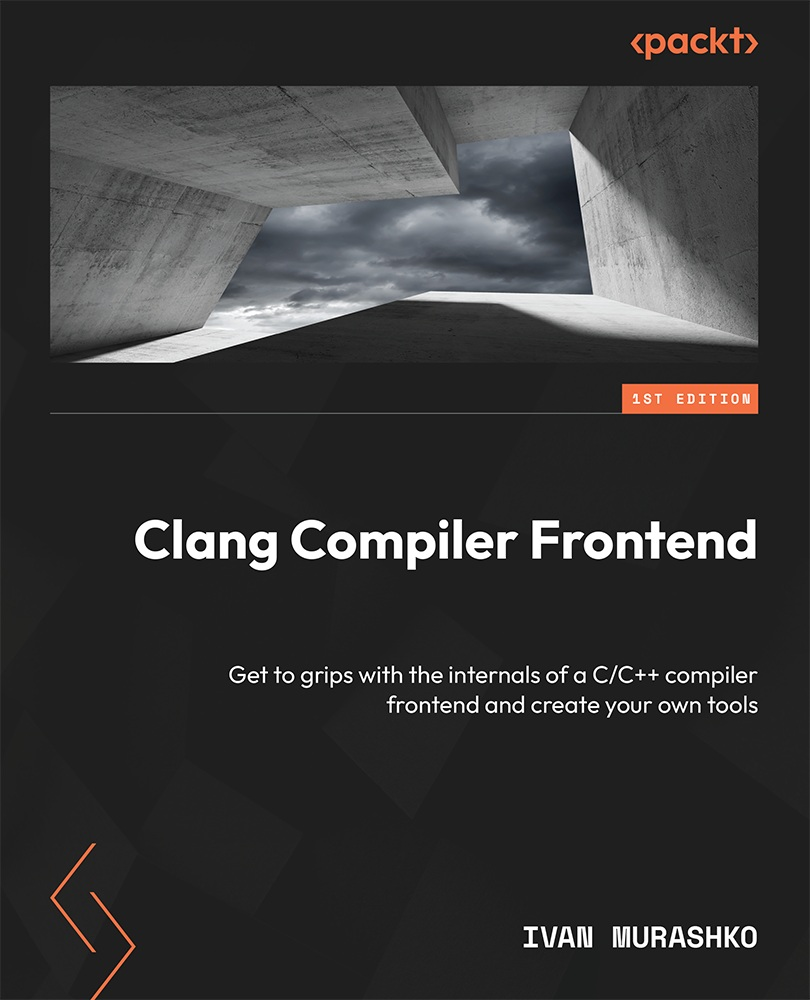
\includegraphics[width=\textwidth,height=\textheight,keepaspectratio]{cover.png}
\begin{tikzpicture}[remember picture, overlay, inner sep=0pt]
\node at (current page.center)
{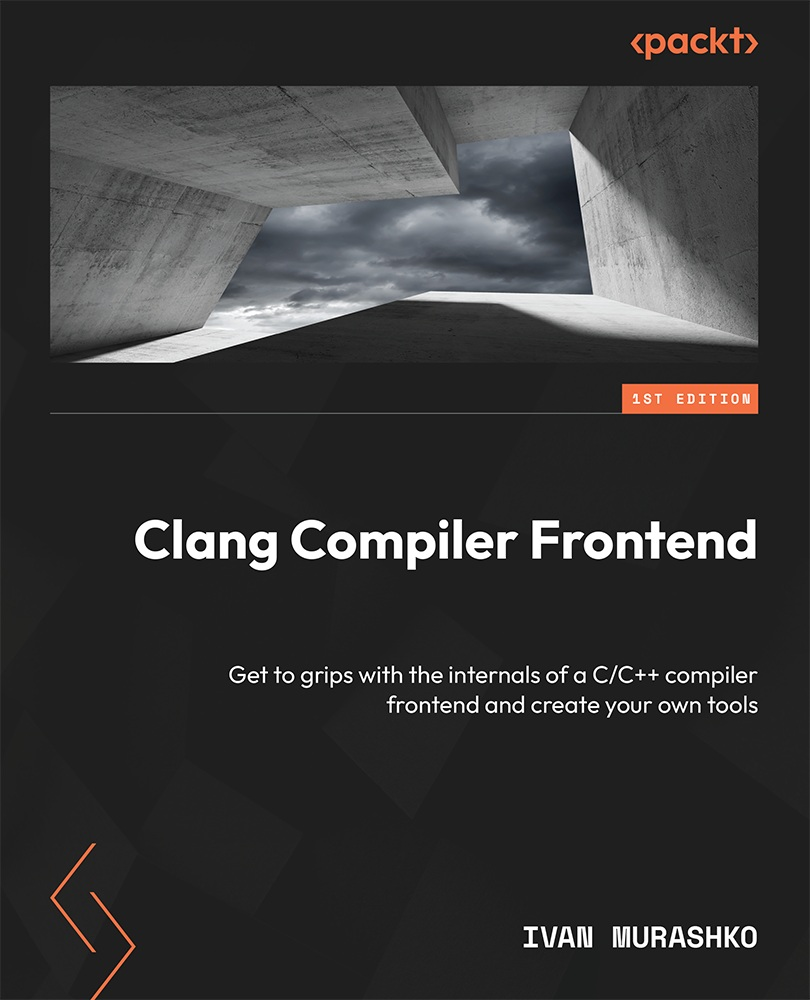
\includegraphics[width=\paperwidth, keepaspectratio=false]{cover.png}};
\end{tikzpicture}
\newpage
\thispagestyle{empty}
\huge
\textbf{Clang Compiler Frontend}
\\[9pt]
{\Large Get to grips with the internals of a C/C++ compiler frontend and create your own tools}
\\[9pt]
\normalsize
作者: Ivan Murashko
\\[8pt]
\normalsize
译者:\href{https://github.com/xiaoweiChen/Clang-Compiler-Frontend}{陈晓伟}
\\[8pt]
\end{center}

\newpage

\pagestyle{empty}
\tableofcontents
\newpage


\setsecnumdepth{section}

\myPart{}{关于作者}{about-the-author.tex}
\newpage

\myPart{}{关于评审}{about-the-reviewer.tex}
\newpage

\myPart{}{前言}{preface.tex}
\newpage

\myPart{第一部分}{Clang Setup and Architecture}{part1/title.tex}
\newpage

\myChapter{第1章}{Environment Setup}{part1/chapter1/0.tex}
\mySubsection{1.1.}{Technical requirements}{part1/chapter1/1.tex}
\mySubsection{1.2.}{Getting to know LLVM}{part1/chapter1/2.tex}
\mySubsection{1.3.}{Source code compilation}{part1/chapter1/3.tex}
\mySubsection{1.4.}{Test project - syntax check with a Clang tool}{part1/chapter1/4.tex}
\mySubsection{1.5.}{总结}{part1/chapter1/5.tex}
\mySubsection{1.6.}{扩展阅读}{part1/chapter1/6.tex}
\newpage

\myChapter{第2章}{Clang Architecture}{part1/chapter2/0.tex}
\mySubsection{2.1.}{Technical requirements}{part1/chapter2/1.tex}
\mySubsection{2.2.}{Getting started with compilers}{part1/chapter2/2.tex}
\mySubsection{2.3.}{Clang driver overview}{part1/chapter2/3.tex}
\mySubsection{2.4.}{Clang fronted overview}{part1/chapter2/4.tex}
\mySubsection{2.5.}{总结}{part1/chapter2/5.tex}
\mySubsection{2.6.}{扩展阅读}{part1/chapter2/6.tex}
\newpage

\myChapter{第3章}{Clang AST}{part1/chapter3/0.tex}
\mySubsection{3.1.}{Technical requirements}{part1/chapter3/1.tex}
\mySubsection{3.2.}{AST}{part1/chapter3/2.tex}
\mySubsection{3.3.}{AST traversal}{part1/chapter3/3.tex}
\mySubsection{3.4.}{Recursive AST visitor}{part1/chapter3/4.tex}
\mySubsection{3.5.}{AST matchers}{part1/chapter3/5.tex}
\mySubsection{3.6.}{Explore Clang AST with clang-query}{part1/chapter3/6.tex}
\mySubsection{3.7.}{Processing Ast in the case of errors}{part1/chapter3/7.tex}
\mySubsection{3.8.}{总结}{part1/chapter3/8.tex}
\mySubsection{3.9.}{扩展阅读}{part1/chapter3/9.tex}
\newpage

\myChapter{第4章}{Basic Libraries and Tools}{part1/chapter4/0.tex}
\mySubsection{4.1.}{Technical requirements}{part1/chapter4/1.tex}
\mySubsection{4.2.}{LLVM coding style}{part1/chapter4/2.tex}
\mySubsection{4.3.}{LLVM basic libraries}{part1/chapter4/3.tex}
\mySubsection{4.4.}{Clang basic libraries}{part1/chapter4/4.tex}
\mySubsection{4.5.}{LLVM supporting tools}{part1/chapter4/5.tex}
\mySubsection{4.6.}{Clang plugin project}{part1/chapter4/6.tex}
\mySubsection{4.7.}{总结}{part1/chapter4/7.tex}
\mySubsection{4.8.}{扩展阅读}{part1/chapter4/8.tex}
\newpage

\myPart{第二部分}{Clang Tools}{part2/title.tex}
\newpage

\myChapter{第5章}{Clang-Tidy Linter Framework}{part2/chapter5/0.tex}
\mySubsection{5.1.}{Technical requirements}{part2/chapter5/1.tex}
\mySubsection{5.2.}{Overview of Clang-Tidy and usage examples}{part2/chapter5/2.tex}
\mySubsection{5.3.}{Clang-Tidy's internal design}{part2/chapter5/3.tex}
\mySubsection{5.4.}{Custom Clang-Tidy check}{part2/chapter5/4.tex}
\mySubsection{5.5.}{总结}{part2/chapter5/5.tex}
\mySubsection{5.6.}{扩展阅读}{part2/chapter5/6.tex}
\newpage

\myChapter{第6章}{Advanced Code Analysis}{part2/chapter6/0.tex}
\mySubsection{6.1.}{Technical requirements}{part2/chapter6/1.tex}
\mySubsection{6.2.}{Static analysis}{part2/chapter6/2.tex}
\mySubsection{6.3.}{CFG}{part2/chapter6/3.tex}
\mySubsection{6.4.}{Custom CFG check}{part2/chapter6/4.tex}
\mySubsection{6.5.}{CFG on Clang}{part2/chapter6/5.tex}
\mySubsection{6.6.}{Brief description of Clang analysis tools}{part2/chapter6/6.tex}
\mySubsection{6.7.}{Knowing the limitations of analysis}{part2/chapter6/7.tex}
\mySubsection{6.8.}{总结}{part2/chapter6/8.tex}
\mySubsection{6.9.}{扩展阅读}{part2/chapter6/9.tex}
\newpage

\myChapter{第7章}{Refactoring Tools}{part2/chapter7/0.tex}
\mySubsection{7.1.}{Technical requirements}{part2/chapter7/1.tex}
\mySubsection{7.2.}{Custom code modification tool}{part2/chapter7/2.tex}
\mySubsection{7.3.}{Clang-Tidy as a code modification tool}{part2/chapter7/3.tex}
\mySubsection{7.4.}{Code modification and Clang-Format}{part2/chapter7/4.tex}
\mySubsection{7.5.}{总结}{part2/chapter7/5.tex}
\mySubsection{7.6.}{扩展阅读}{part2/chapter7/6.tex}
\newpage

\myChapter{第8章}{IDE Support and Clangd}{part2/chapter8/0.tex}
\mySubsection{8.1.}{Technical requirements}{part2/chapter8/1.tex}
\mySubsection{8.2.}{Language Server Protocol}{part2/chapter8/2.tex}
\mySubsection{8.3.}{Environment setup}{part2/chapter8/3.tex}
\mySubsection{8.4.}{LSP demo}{part2/chapter8/4.tex}
\mySubsection{8.5.}{Integration with Clang tools}{part2/chapter8/5.tex}
\mySubsection{8.6.}{performance optimizations}{part2/chapter8/6.tex}
\mySubsection{8.7.}{总结}{part2/chapter8/7.tex}
\mySubsection{8.8.}{扩展阅读}{part2/chapter8/8.tex}
\newpage

\myPart{第三部分}{附录}{part3/title.tex}
\newpage

\myChapter{附录A}{Compilation Database}{part3/appendix-A/0.tex}
\mySubsection{A.1.}{Compilation database definition}{part3/appendix-A/1.tex}
\mySubsection{A.2.}{CDB ceration}{part3/appendix-A/2.tex}
\mySubsection{A.3.}{Clang tools and a CDB}{part3/appendix-A/3.tex}
\mySubsection{A.4.}{扩展阅读}{part3/appendix-A/4.tex}
\newpage

\myChapter{附录B}{Build Speed Optimization}{part3/appendix-B/0.tex}
\mySubsection{B.1.}{Technical requirements}{part3/appendix-B/1.tex}
\mySubsection{B.2.}{Precompiled headers}{part3/appendix-B/2.tex}
\mySubsection{B.3.}{Clang modules}{part3/appendix-B/3.tex}
\mySubsection{B.4.}{扩展阅读}{part3/appendix-B/4.tex}
\newpage

\myChapter{附录C}{Bibliography}{part3/appendix-C/0.tex}
\newpage
